\documentclass[10pt]{scrreprt}
\usepackage[utf8]{inputenc}
\usepackage{amsfonts}
\usepackage{amsmath}
\usepackage{amssymb}
\usepackage{commath}
\usepackage[ngerman]{babel}
\usepackage{enumitem}
\usepackage{booktabs}
\usepackage{longtable}
\usepackage{relsize}
\usepackage{pgfplots}
\usepackage{csvsimple}
\usepackage{pgfplotstable}
\usepackage{siunitx}
\usepackage{fancyhdr}
\usepackage{color}
\usepackage{float}
\usepackage{listings}
\usepackage{graphicx}
\usepackage{subcaption}
\usepackage[europeanresistors]{circuitikz}
\usepackage{multirow}
\usepackage{tikz-timing}

\def\timingwidth{4}
\def\timingheight{1}

\newcommand\tikzmark[1]{%
  \tikz[overlay,remember picture] \coordinate (#1);}

\definecolor{mygreen}{RGB}{28,172,0} % color values Red, Green, Blue
\definecolor{mylilas}{RGB}{170,55,241}


\lstset{language=Matlab,%
%basicstyle=\color{red},
breaklines=true,%
morekeywords={matlab2tikz},
keywordstyle=\color{blue},%
morekeywords=[2]{1}, keywordstyle=[2]{\color{black}},
identifierstyle=\color{black},%
stringstyle=\color{mylilas},
commentstyle=\color{mygreen},%
showstringspaces=false,%without this there will be a symbol in the places where there is a space
%numbers=left,%
%numberstyle={\tiny \color{black}},% size of the numbers
%numbersep=9pt, % this defines how far the numbers are from the text
emph=[1]{for,end,break},emphstyle=[1]\color{red}, %some words to emphasise
%emph=[2]{word1,word2}, emphstyle=[2]{style},
}

\setlength\parindent{0pt}

\setcounter{chapter}{3}
\setcounter{secnumdepth}{2}
\setcounter{section}{1}

\pagestyle{fancy}
\fancyhf{}
\lhead{GPET Versuch 12}
\rhead{Tim Luchterhand, Paul Nykiel}
\cfoot{\thepage}

\author{Tim Luchterhand, Paul Nykiel \protect\\ tim.luchterhand@uni-ulm.de, paul.nykiel@uni-ulm.de}
\title{GPET Versuch 12 --- Würfeln mit Eccles \& Jordan}
\subtitle{Gruppe: Dienstag14}

\begin{document}
    \maketitle

    \section{8 Bit-Asynchronzähler}
    Wie Sie feststellen konnten, erfordert der Aufbau eines einzelnen Flip-Flops aus Logikgattern
    einen erheblichen Schaltungsaufwand. Um auch komplexer Schaltwerke realisieren zu
    können, verwenden wir ab jetzt die integrierten D-Flip-Flops im Bereich (F) des \textit{Digital-
    Boards}. Entfernen Sie für diesen Versuch zunächst alle Jumper. Sie benötigen lediglich
    den Jumper für die Wahl des CLK -Tasters als Takteingangs und eine Verbindung des
    ersten Flip-Flops des Zählers mit dem zentralen Taktsignal.

    \subsection{Aufbau}
    Bauen Sie einen 8 Bit-Asynchronzähler nach dem Prinzip aus Vorbereitungsfrage 2.3 auf.
    Verwenden Sie den CLK -Taster zur Erzeugung eines Taktpulses und überprüfen Sie die
    Funktionalität. Um die höherwertigen Bits zu überprüfen können Sie den Zähler mit den
    SET -Tastern auch vorinitialisieren. Zeigen Sie anschließend den Aufbau Ihrem Tutor.

    \subsection{Zwischenwerte}
    Betrachten Sie nun die Ausgänge des Zählers auf dem Oszilloskop. Setzten Sie zunächst
    das Oszilloskop mittels \framebox{Default Setup} zurück. Verbinden Sie anschließend die Flip-Flops
    mit den Ausgängen 0-7 des im Bereich (G) und schließen Sie die Digitaleingänge des
    Oszilloskops an die Stiftleiste an. Aktivieren Sie im die Eingänge $D_0 -D_7$ im \framebox{Digital}
    Menü und gruppieren Sie diese als Hexadezimal-Bus. Achten Sie darauf, dass die richtigen
    Schwellwerte für die digitalen Eingänge (CMOS, 2,5 V) eingestellt sind. Stellen Sie zuletzt
    den \framebox{Trigger} auf einen geeigneten Eingang ein und wählen Sie die wechselnde Flanke,
    um sowohl bei steigender als auch bei fallender Flanke ein Triggerevent auszulösen. Der
    Triggermodus sollte mittels \framebox{Mode/Coupling} auf Normal gestellt werden, da im
    Auto-Modus auch bei fehlendem Triggerimpuls eine Aktualisierung durchgeführt wird.
    Schauen Sie sich den Übergang vom Zählerstand $0111\ 1111_\text{bin}$ ($127_\text{dec}$ bzw. $7F_\text{hex}$) zum
    Zählerstand $1000\ 0000_\text{bin}$ ($128_\text{dec}$ bzw. $80_\text{hex}$) an. Tragen Sie die Zwischenzustände des
    Asynchronzählers in das Timing-Diagramm in Abbildung 18 ein und nehmen Sie einen
    Screenshot vom Oszilloskop in Ihr Protokoll mit auf. Was ist der Grund für diese
    Zwischenzustände?

    %\begin{figure}[H]
    %    \begin{tikztimingtable}
    %        [timing/coldist=2pt,
    %        xscale=1,yscale=2]
    %        $D_7$ & L\\
    %        $D_6$ & H\\
    %        $D_5$ & H\\
    %        $D_4$ & H\\
    %        $D_3$ & H\\
    %        $D_2$ & H\\
    %        $D_1$ & H\\
    %        $D_0$ & H\\
    %        HEX   & [d] D{7F} 8{D{}}\\
    %        \extracode
    %        \tablegrid[black!25]
    %    \end{tikztimingtable}
    %    \caption{Vervollständigen Sie das Timing-Diagramm der ungetakteten Latches.}
    %    \label{fig:TimeGetaktetesLatch}
    %\end{figure}

    \paragraph{Protokoll}
    $ $
    \begin{figure}[H]
        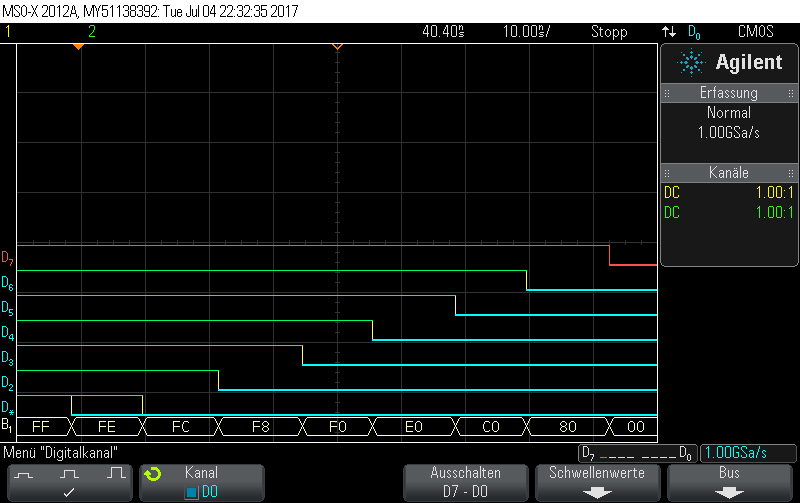
\includegraphics[width=\textwidth]{scope_3.png}
        \caption{Timing Diagramm}
    \end{figure}
    \begin{figure}[H]
        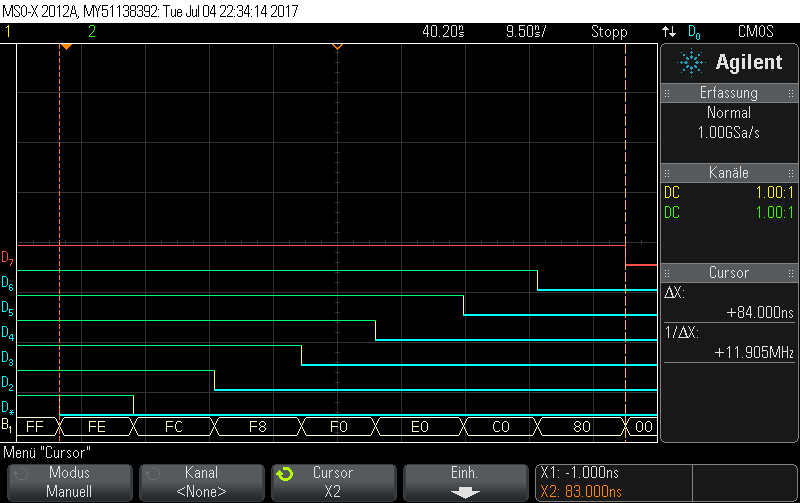
\includegraphics[width=\textwidth]{scope_4.png}
        \caption{Verzögerung}
        \label{fig:gesLaufzeit}
    \end{figure}

    Jedes Flip-Flop hat eine gewisse Laufzeit. Diese Laufzeiten sind in den Scrennshots
    als Verschiebung zwischen den einzelnen Flanken zu erkennen.
    Da beim Asynchronzähler alle Flip-Flops in Reihe geschalten sind, addieren
    sich die Laufzeiten auf. Die Zwischenzustände treten auf, wenn teilweise
    Flip-Flops noch nicht geschalten wurden, die vorrangegangenen Flip-Flops aber
    bereits in einem neuen Zustand sind.

    \subsection{Gatterlaufzeit}
    Bestimmen Sie Zeit bis ein neuer (korrekter) Zählerstand an den Ausgängen anliegt und
    errechnen Sie daraus die Laufzeitverzögerung eines D-Flip-Flops.

    Wie in Grafik~\ref{fig:gesLaufzeit} zu erkennen, besitzt der Asynchronzähler
    eine Gessamtlaufzeit von $t_{ges} = 84\si{n\second}$. Daraus lässt sich die Laufzeit eines
    einzelnen Flip-Flops berechen:

    \begin{equation*}
        t_{Flip-Flop} = \frac{t_{ges}}{8} = 10.5\si{n\second}
    \end{equation*}

    \section{4 Bit-Synchronzähler}
    Setzten Sie für diesen Versuch alle vertikalen Jumper auf das \textit{Digital-Board}. Damit werden
    alle Flip-Flops mit dem zentralen Taktsignal versorgt. Verwenden Sie weiterhin den CLK -
    Taster als Takteingang.

    \subsection{Aufbau}
    Bauen Sie nun einen 4 Bit-Synchronzähler mit der Zählreihenfolge $0 \rightarrow 3 \rightarrow 6 \rightarrow 9 \rightarrow 12
    \rightarrow 0 \rightarrow \ldots$ auf und überprüfen Sie die Funktionalität. Verwenden Sie dazu die Ergebnisse
    von Vorbereitungsfrage 2.4. Zeigen Sie den Aufbau Ihrem Tutor.

    \subsection{Übergänge}
    Betrachten Sie auch hier die vier Bits des Zählers auf dem Oszilloskop. Schauen Sie sich
    die Übergänge der Zählerstände an. Im Gegensatz zum Asynchronzähler sollten die
    Übergänge beim Synchronzähler gleichzeitig stattfinden. Dennoch werden Sie bei mehrfacher
    Wiederholung des Versuches feststellen, dass die Übergänge unter Umständen zu minimal
    unterschiedlichen Zeitpunkten stattfinden. Dies ist auf verschiedene Ursachen zurückzuführen.
    Neben leicht unterschiedlichen Laufzeiten der einzelnen D-Flip-Flops hängt dies
    primär mit der Datenerfassung der digitalen Eingänge des Oszilloskops zusammen. Ein
    limitierender Faktor ist die minimale Zeitauflösung des Oszilloskops. Was ist die maximale
    Zeitliche Auflösung des Oszilloskops, oder anders ausgedrückt der minimale Laufzeitunterschied
    den Sie beobachten können?

    \vspace{.5cm}

    Zudem stellt der digitale Eingang das Signal stark idealisiert dar, da ein einfacher
    Schwellwertvergleich vorgenommen wird. Liegt das Eingangssignal unterhalb des eingestellten
    Referenzpegels (bei CMOS 2,5 V), so wird eine 0 erkannt, oberhalb eine 1. Tatsächlich
    findet dagegen ein annähernd exponentieller Lade- bzw. Entladevorgang statt, die
    Zeitkonstante wird dabei primär von den parasitären Kapazitäten des folgenden Gatters sowie
    der Eingangskapazität des Oszilloskopeingangs bestimmt.

    \paragraph{Protokol}
    $ $
    \begin{figure}[H]
        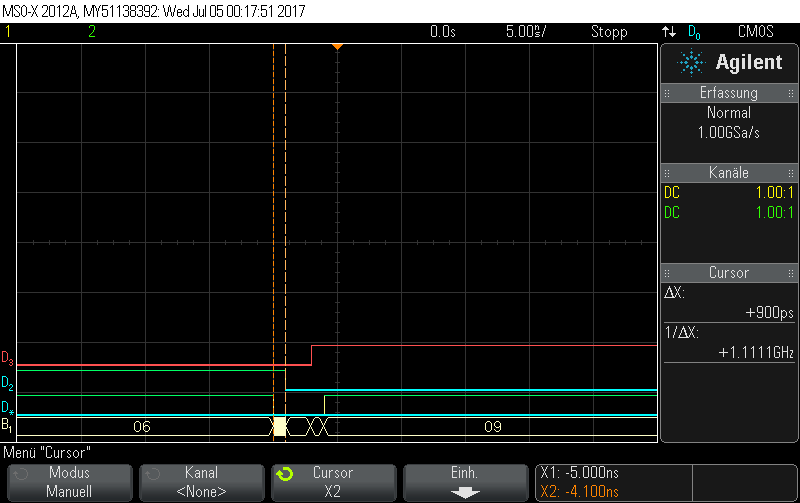
\includegraphics[width=\textwidth]{scope_15.png}
        \caption{4Bit-Synchronzähler}
    \end{figure}
    Aus der Messung ergibt sich:
    \begin{equation*}
        t_{\min} = 900\si{p\second}
    \end{equation*}

    Das Oszilloskop hat also eine maximale zeitliche Auflösung von ca.~$1\si{n\second}$.

    \section{Schieberegister}
    \subsection{Ringzähler}
    Bauen Sie ein 8 Bit-Schieberegister auf, indem Sie die horizontalen Jumper verwenden
    und verbinden Sie den Ausgang des letzten Flip-Flops mit dem Eingang des ersten
    (8 Bit-Ringzähler). Überprüfen Sie die Funktionalität, indem Sie ein beliebiges Bitmu-
    ster \glqq{}durchschieben\grqq{}. Zeigen Sie den Aufbau Ihrem Tutor.

    \subsection{Frequenzteiler}
    Der von Ihnen aufgebaute Ringzähler kann, abhängig vom Anfangszustand des Schieberegisters,
    auch als Frequenzteiler genutzt werden. Betreiben Sie den Ringzähler hierzu
    mit dem Frequenzgenerator aus dem Oszilloskop. Der Frequenzgenerator wird mit der
    Taste \framebox{Wave Gen} aktiviert. Stellen Sie die Form auf Reckteck, die untere Spannung auf
    0 V und die obere Spannung auf 5 V ein, der Arbeitszyklus sollte 50 \% betragen.
    Wenn Sie die richtigen Werte eingestellt haben verbinden Sie den Ausgang Gen. Out
    mit dem BNC-Eingang des Digital-Boards und wählen Sie den BNC-Eingang mit dem
    Jumper aus. Mehrfaches Drücken der Taste \framebox{Wave Gen} aktiviert und deaktiviert das
    Taktsignal. Stellen Sie nun eine Frequenz von 10 Hz ein und stellen Sie diesen Takt sowie
    den Ausgang des letzten Flip-Flops auf dem Oszilloskop dar. Untersuchen Sie die fünf
    Anfangszustände aus Tabelle 4 im Hinblick auf die Frequenzteilung. Messen Sie hierbei
    die Frequenz des Ausgangssignals und leiten Sie daraus die Frequenzteilung sowie den
    Arbeitszyklus ab.

    \paragraph{Protokoll}
    $ $
    \begin{figure}[H]
        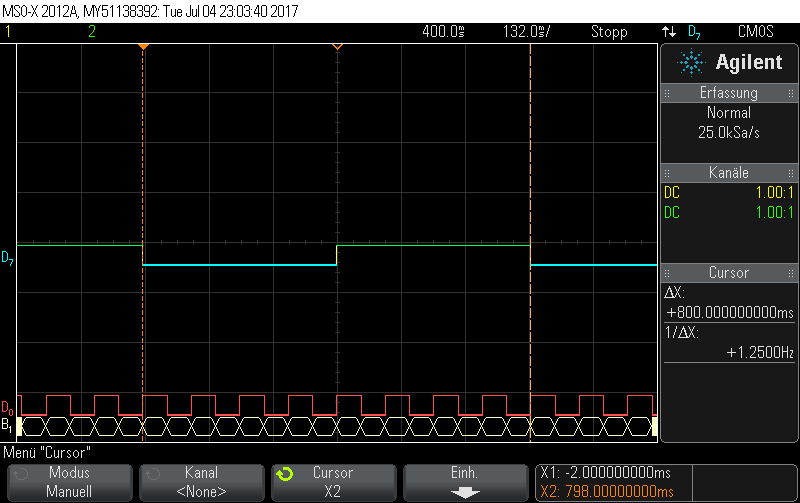
\includegraphics[width=\textwidth]{scope_11.png}
        \caption{Ausgangssignal bei Anfangszustand 11110000}
    \end{figure}
    \begin{figure}[H]
        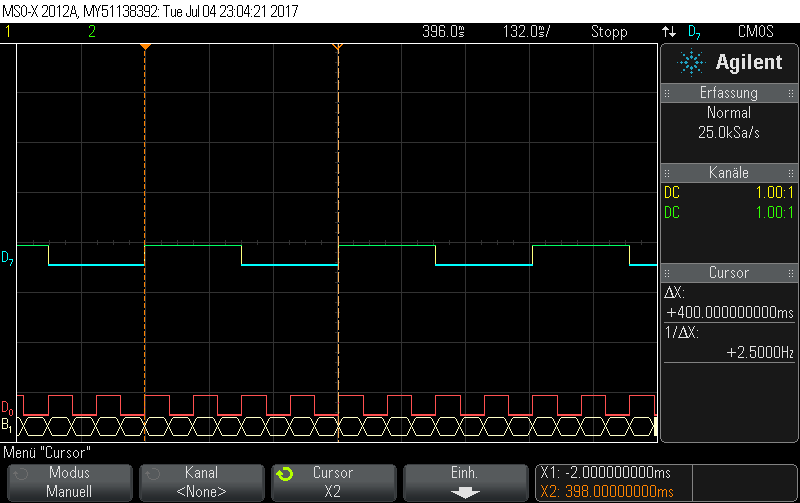
\includegraphics[width=\textwidth]{scope_12.png}
        \caption{Ausgangssignal bei Anfangszustand 11001100}
    \end{figure}
    \begin{figure}[H]
        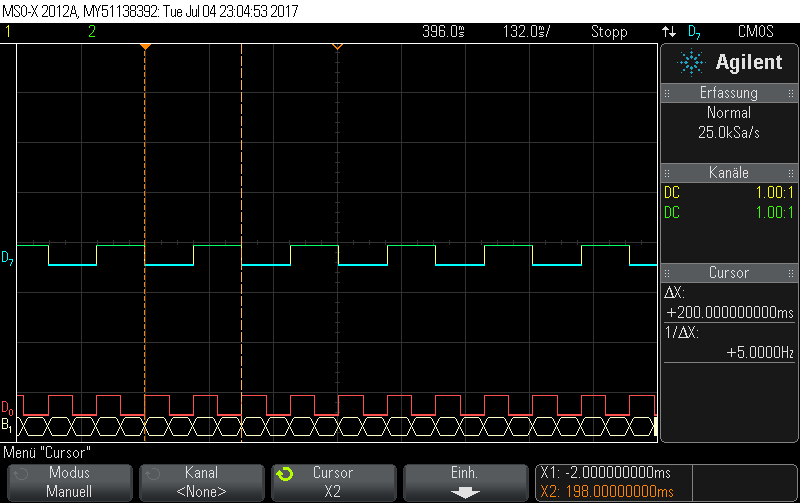
\includegraphics[width=\textwidth]{scope_13.png}
        \caption{Ausgangssignal bei Anfangszustand 10101010}
    \end{figure}
    \begin{figure}[H]
        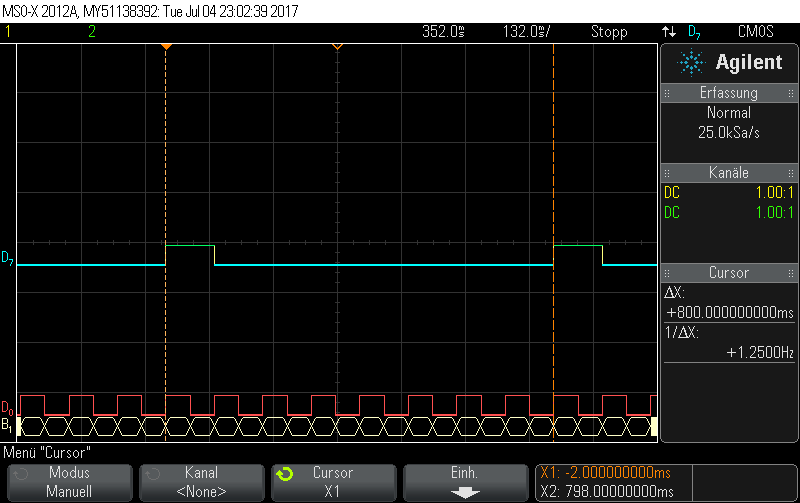
\includegraphics[width=\textwidth]{scope_10.png}
        \caption{Ausgangssignal bei Anfangszustand 10000000}
    \end{figure}
    \begin{figure}[H]
        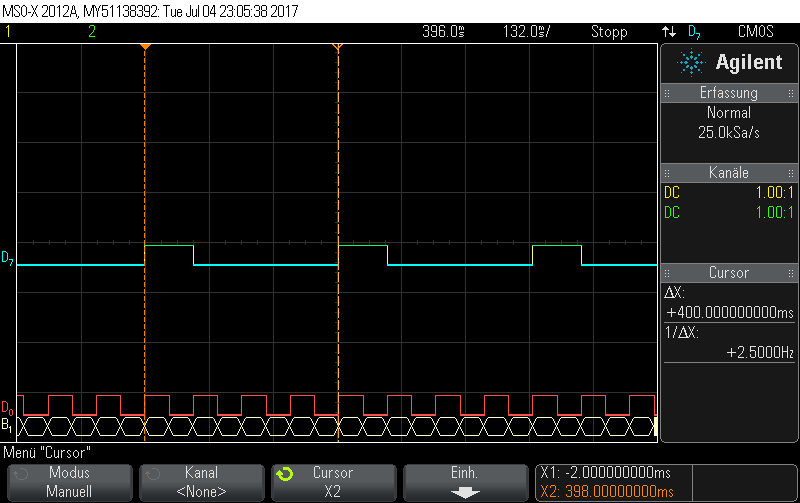
\includegraphics[width=\textwidth]{scope_14.png}
        \caption{Ausgangssignal bei Anfangszustand 10001000}
    \end{figure}
    %TODO Werte auslesen
    \begin{table}[H]
        \centering
        \begin{tabular}{cccc}
            \toprule
            Anfangszustand & Ausgangsfrequenz & Frequenzteilung & Arbeitszyklus\\
            \midrule
            11110000 & $1.25\si{\hertz}$ & 8 & $50\%$\\
            11001100 & $2.5\si{\hertz}$ & 4\ & $50\%$\\
            10101010 & $5\si{\hertz}$ & 2 & $50\%$\\
            10000000 & $1.25\si{\hertz}$ & 8 & $12.5\%$\\
            10001000 & $2.5\si{\hertz}$ & 4 & $25\%$\\
            \bottomrule
        \end{tabular}
        \caption{Messergebnisse des Frequenzteilers.}
        \label{tab:freqteiler}
    \end{table}

    \section{DVB-S Scrambler}
    Bauen Sie das linear rückgekoppelte Schieberegister des DVB-S Scramblers auf, das im
    grau hinterlegten Teil in Abbildung 5 dargestellt ist. Wie kann das Scrambling auf der
    Empfängerseite rückgängig gemacht werden? Wie lautet das Boolesche Gesetz für diesen
    Vorgang? (Tipp: Erinnern Sie sich an den vorherigen Versuch)

    \vspace{.5cm}

    Ermitteln Sie die ersten 20 Werte der PN-Sequenz. Achten Sie auf eine korrekte
    Vorinitialisierung des Registers, die in Abbildung 5 oberhalb jeder Zelle angegeben ist.

    \paragraph{Protokoll}
    Die ersten 20 Zeichen der PN-Sequenz lauten:
    \begin{equation*}
        00000011111101100000
    \end{equation*}
    Um das ursprüngliche Signal wiederherzustellen, muss man das gescrambelte
    Signal mit der bekannten Initialsequenz ver-XODERn. Das resultierende Signal
    wird erneut mit der Initialsequenz ver-XODERt, um das ursprüngliche Signal
    zu erhalten.

    \vspace{.5cm}

    Das Boolsche-Gesetz für diesen Vorgang lautet:
    \begin{equation*}
        a \oplus b \oplus b = a \oplus (b \oplus b) = a \oplus 0 = a
    \end{equation*}

    \section{GPS C/A-Code Generator}
    Bauen Sie den C/A-Code-Generator des GPS-Systems auf, das im grau hinterlegten Teil
    in Abbildung 6 dargestellt ist. Beginnen Sie mit dem G1-Shift-Register nach Abbildung 7
    und dem G2-Shift-Register nach Abbildung 8. Schalten Sie als letztes die Verknüpfungen
    zur Generierung der $G_i$-Sequenz gemäß Abbildung 6. In Tabelle 5 finden Sie die
    entsprechenden Werte für die Phase-Select-Logic der Satelliten 5, 13 und 17. Ermitteln Sie für
    diese Satelliten jeweils die ersten 10 Werte der PN-Sequenz. Beide Register müssen dabei
    jeweils mit Einsen vorinitialisiert werden.
    \begin{table}[H]
        \centering
        \begin{tabular}{ccc}
            \toprule
            Satellit & Phase-Select-Logic & PN-Sequenz\\
            \midrule
            $5$ & $1 \oplus 9$ & $1001011011$\\
            $13$ & $6 \oplus 7$ & $1111110100$\\
            $17$ & $1 \oplus 4$ & $1001101110$\\
            \bottomrule
        \end{tabular}
        \caption{GPS C/A Code}
        \label{tab:GPS}
    \end{table}
\end{document}
